\chapter{Dynamical Systems}
\label{chap:ch3}

\section{Defining Ordinary Differential Equations}
\begin{definition}
	\textit{An \textbf{ordinary differential equation} is an equation of an unknown function of \textbf{one} variable. This can be expressed as a function \textbf{of} this unknown function, its corresponding variable and its various derivatives}.
\end{definition}
Its general form looks something like:
\begin{equation}\label{ODE}
	F(t,y(t),y'(t),....,y^{(n)}(t))=0,
\end{equation}
Where $y(t)$ is the unknown function of independent variable $t$ and $F : \Omega \rightarrow \mathbb{R},  \\ \Omega \subseteq \mathbb{R}^{n+1}$.

This would be what's called the implicit form of the differential equation.

\begin{definition}
	\textit{The \textbf{order} of an ODE is the highest order of the derivative present in the equation.}
\end{definition}
In our case, the order is $n$.
If, however $F$ satisfies the regularity condition \textbf{of the implicit function theorem} then the equation can be written in a much more digestible form.

The \textbf{implicit function theorem} allows one to convert a relation (implicit form) to functions of some variables. These functions may not be unique, but together, their graph may locally satisfy the relation.

As an example: The relation for a cardioid cannot be expressed as a sole function, we'd instead need the union of the graph of two separate functions for expressing it.
(si aici gen faci tu niste graphuri cu maple sau alte d-astea vezi cum faci virtual machineu ala sau mergi la faculta la un pc cu maple si iti faci lista cu ce vrei sa graphuiesti)

\textbf{Reminder}: A function $f(x)$ is continuously differentiable if $\exists f'(x)$ and $f'(x) \in C^n$ where $n>=0$

\begin{theorem}
	Let $F:D \subseteq \mathbb{R}^{n+1}\rightarrow\mathbb{R}$ be a continuously differentiable function with the relation that $F(t,y(t),y'(t),....,y^{(n)}(t))=0$. Let us express a point in the set $\mathbb{R}^{n+1} =\mathbb{R}\bigtimes\mathbb{R}^n$ as (t, \textbf{Y}) = $(t, y,y', \dots, y^{ (n) })$ and fix one such point s.t. $F(t, \textbf{Y})=0$.
	So $\exists \square_{(t, \textbf{Y})} \ni U \bigtimes V \subseteq D$ s.t. $F \in C^1(U\bigtimes V)$ and $\frac{\partial F}{\partial y}(t, \textbf{Y}) \neq 0.$ Then this means $ \exists \square_{t} \ni U_0 \subseteq U$,
	$\square_{\textbf{Y}} \ni V_0 \subseteq V$ and a function $f : U_0 \rightarrow V_0$ s.t. $f(t) = \textbf{Y}$ and $F(t,f(t))=0, \forall t \in U_0; f \in C^1(U_0)$ and $\frac{\partial f}{\partial t_i} = - \frac{\frac{\partial F}{\partial t_i}(t,f(t))}{\frac{\partial F}{\partial y}(t,f(t))}, \forall i = \overline{1,n} , \forall t \in U_0$ and $F \in C^1(U \bigtimes V),K \in N^* \Rightarrow f \in C^K(U_0).$
\end{theorem}

\hfill\break
//TODO : proof: trust me bro
\hfill\break

So restricting the domain $\Omega$ to one that allows the implicit form to be represented as a function of the form
\begin{equation}\label{implicit_func_theorem}
	y^{(n)}(t)=f(t,y(t),y'(t),...,y^{(n-1)}(t))
\end{equation}
would yield what's called the \textbf{explicit} form of the ODE.

A \textbf{solution} is an expression of the unknown function $y(t)$ which satisfies the relation
$y^{(n)}(t) = f(t,y(t),y'(t),\dots,y^{(n-1)}(t))$. A \textbf{general solution} includes all of these functions and usually has some constants of integration in the expression, while a \textbf{particular solution} doesn't have them.

A particular solution is usually found if we also have some initial conditions given for the unknown function, like $y(a)=b, y'(a)=c$ for some $a,b,c \in \mathbb{R}$.
Or, more formally:

\begin{definition}
	A function $y:I \rightarrow \mathbb{R}$ is a solution of the equation \ref{ODE} if the following conditions are met:

	1. $I \subseteq \mathbb{R}$ is nondegeneate interval. ($|I|>1$)

	2. $y \in C^n(I)$ and $(t,y(t), y'(t), \dots, y^{(n)}(t)) \in D_f, \forall t \in I$.

	3. $y^{(n)}(t)= f(t,y(t),y'(t),\dots,y^{ (n-1) }(t)), \forall t \in I$. ( \ref{implicit_func_theorem} is satisfied)

\end{definition}

\section{Forming Ordinary Differential Equation systems}
We may take a sequence of such first order ordinary differential equations to form a system:
\begin{equation}\label{3.2.1}
	\begin{cases}
		y'_1(t) = f_1(t,y_1(t),y_2(t),\dots,y_n(t)) \\
		y'_2(t) = f_2(t,y_1(t),y_2(t),\dots,y_n(t)) \\
		\vdots                                      \\
		y'_n(t) = f_n(t,y_1(t),y_2(t),\dots,y_n(t))
	\end{cases}
\end{equation}

Constructing $y: D \subseteq \mathbb{R} \rightarrow \mathbb{R}^n, f : D_f \subseteq \mathbb{R}^{n+1} \rightarrow \mathbb{R}^n$ and denoting \\
$y(t)= (y_1(t), \dots, y_n(t))$ and $f(t,y_1(t),\dots,y_n(t)) = (f_1,\dots,f_n)$ we get what is called the \textbf{vector form} of the system \ref{3.2.1}.

\begin{equation}\label{3.2.2}
	y'(t) = f (t, y(t))
\end{equation}

\begin{definition}
	For a function $y:D \subseteq \mathbb{R} \rightarrow \mathbb{R}^n$ , $|D| > 1$, if $y \in C^1(D,\mathbb{R}^n)$, and $y'(t) = f(t,y(t)), \forall t \in D \Rightarrow$ $y$ is a \textbf{solution of the system} \ref{3.2.2}.
\end{definition}

\begin{definition}
	An \textbf{autonomous equation} is a differential equation that does not explicitly depend on time, but is instead only defined by the relation between the function itself and its derivatives, so an equation of the form
	\begin{equation}\label{eq:3.2.3}
		f(y^{(n)}(t), y^{(n-1)}(t), \dots, y(t))= 0
	\end{equation}
	That is not to say, the function itself does not depend on time, but rather the independent variable $t$ does not explicitly appear in the equation.
\end{definition}

One more famous such example is the equation for the damped oscillator
\begin{equation}\label{eq:3.2.4}
	\ddot{x} + 2\gamma\dot{x} + \omega^2x = 0.
\end{equation}

Where:
\begin{itemize}
	\item $\gamma$ is the damping factor, meaning how quickly the oscillations of the system decay due to loss of momentum (caused by air resistance or friction)

	\item $\omega$ represents the angular (natural) frequency the oscillator would have, were it not to be affected by damping, defined by
		$\omega = \sqrt{\frac{k}{m}}$; where $k$ is the \textbf{elastic stiffness coefficient} of the spring and $m$ the mass.
\end{itemize}

In addition, a frequently used notation in physics is
$\dot{x} = \frac{d}{dt}x$ , $\ddot{x}=\frac{d^2}{dt^2}x$

That equation is a \textbf{linear} homogenous equation with constant coefficients (hence autonomous), which is pretty nice to work with. Their general form would be:
\begin{equation}\label{lin_hom_eq_const}
	a_0 x + a_1\dot{x}+ \dots +a_{n} x^{(n)} = 0
\end{equation}

Finding exact solutions, though, can be done by using some nice properties of Euler's exponential function $e^{rt}$.

Introducing the notion of \textbf{operators} would help in writing this next section.

\begin{definition}
	$D = \frac{d}{dt}$ is the \textbf{derivation operator}:
	$D^n = \frac{d^n}{dt^n}$, so $D^nu = D^n(u) =\frac{d^nu}{dt^n}$ where $u=u(t)$ and (related to \ref{lin_hom_eq_const}): \par
	\hspace{20pt} $L = a_0 + a_1D + \dots + a_nD^n$ \par
	\hspace{20pt} is the \textbf{linear differential operator of order n}. Meaning \ref{lin_hom_eq_const} $\iff Lx=0$.
\end{definition}

We now can; just by pure Ansatz; assume the solutions take the form $e^{rt}$ for some (yet unknown) $r$'s. Because the exponential is so easy to work with when it comes to taking derivatives - a.k.a. : $D^n(e^{rt})=r^ne^{rt}$, so its derivatives are proportional to itself, meaning no new $t$'s are introduced - substituting back into \ref{lin_hom_eq_const} yields
\begin{gather*}
	Le^{rt} = a_0 e^{rt} + a_1 De^{rt} + \dots +a_{n} D^ne^{rt} = 0      \\
	\Updownarrow \\
	a_0 e^{rt}+a_1re^{rt} + \dots + a_nr^ne^{rt} =0 \\
	\Updownarrow \\
	a_0 + a_1r + \dots + a_nr^n =0
\end{gather*}
The left-hand-side is the \textbf{characteristic polynomial} of the linear equation.
\begin{equation}\label{lin_eq_char_poly}
	p(r) = a_1r + \dots + a_nr^n
\end{equation}
Notice that $L = p(D)$. \\
So now it all comes down to finding its roots $r$.

Case \rom{1}: A \textbf{unique, real} root found:

now $e^{rt}$ is a \textbf{fundamental solution} for $Le^{rt}=0$

Case \rom{2}: A \textbf{unique, complex} root found:

say it has the form $r = \lambda \pm i\mu, \mu \neq 0$. \\
By Euler's formula:
\begin{equation}\label{euler}
	e^{rt} = e^{(\lambda + i\mu)t} = e^{\lambda t} \cdot e^{i \mu t}  =  e^{\lambda t} \cdot [\text{cos}(\mu t) + i \text{sin}(\mu t)]
\end{equation}

So $e^{\lambda t}\text{cos}(\mu t)$ and $e^{\lambda t}\text{sin}(\mu t)$ are both fundamental solutions for $Lx=0$.

\textbf{Proof}: \par
Since $a_i \in \mathbb{R}, \forall i=\overline{1,n}$ in $p \implies p(\overline{r})=\overline{p(r)}, \forall r \in \mathbb{C}$, hence, just like 2AM coffee and the exam session, complex roots of $p$ always come in pairs. They both satisfy:
\begin{equation}\label{lin_op_solution}
	Le^{(\lambda \pm i \mu)} = 0
\end{equation}

But since our $x : \mathbb{R} \rightarrow \mathbb{R}$ we're looking for \textbf{real} valued solutions.
Because $\mu \in \mathbb{R}$ the following properties hold equivalently for $\lambda + i\mu$ and for $\overline{\lambda + i\mu}=\lambda - i\mu$ so I'll only write $\lambda \textbf{+} i \mu$ for simplicity. By \ref{euler}:
\begin{equation}\label{eulers_real_and_imaginary}
	\text{Re}(e^{rt})=e^{\lambda t} \cdot \text{cos}(\mu t), \hspace{2cm}    \text{Im}(e^{rt}) = e^{\lambda t} \cdot \text{sin}(\mu t).
\end{equation}
But (\textbf{reminder})
\begin{gather}\label{real_imag_another_way_to_write}
	\text{Re}(c)= \frac{c+\overline{c}}{2}, \hspace{2cm}
	\text{Im}(c) = \frac{c-\overline{c}}{2i}
\end{gather}
\begin{gather*}
	\forall c \in \mathbb{C}
\end{gather*}

\newcommand\firstConclusion{\stackrel{\mathclap{\normalfont\mbox{\ref{eulers_real_and_imaginary}, \ref{real_imag_another_way_to_write}}}}{=\joinrel=\joinrel=\joinrel=\joinrel=\joinrel=}}

\newcommand\byDistributivity{\stackrel{\mathclap{\normalfont\mbox{dist.}}}{=\joinrel=\joinrel=}}

\newcommand\operatorSatisfy{\stackrel{\mathclap{\normalfont\mbox{\ref{lin_op_solution}}}}{=\joinrel=}}

Using these three conclusions we get:
\begin{align*}
	L(e^{\lambda t} \cdot \text{cos}(\mu t)) \firstConclusion
	L\left(\frac{e^{rt}+e^{\overline{r}t}}{2} \right) \byDistributivity
	\frac{1}{2} \left( Le^{rt} + Le^{\overline{r}t} \right) \operatorSatisfy 0 , \\
	L(e^{\lambda t} \cdot \text{sin}(\mu t)) \firstConclusion
	L\left(\frac{e^{rt}-e^{\overline{r}t}}{2i} \right) \byDistributivity
	\frac{1}{2i} \left( Le^{rt} - Le^{\overline{r}t} \right) \operatorSatisfy 0 ,
\end{align*}

In conclusion, if $Le^{ct}=0$ for some $c \in \mathbb{C} \implies L\text{Re}(e^{ ct })= L\text{Im}(e^{ct})=0, \\
\text{for } \text{Re}(e^{ct}), \text{Im}(e^{ct}) \in \mathbb{R}$.
Moreover, the same can be said for $e^{\overline{c}t}$. \qed

Now something let's say... \textbf{fundamental} (hehe) about these solutions, is they have to be linearly independent to each other. Meaning the only solution for
\begin{equation}\label{liniar_independece}
	c_1 x_1+c_2 x_2 + \dots + c^n x^n = 0
\end{equation}
is the trivial solution $c_1=c_2=\dots=c_n=0$ where $x_i$ are the fundamental solutions of the system.

So the reason I've emphasized "\textbf{unique}" in the first 2 cases was because if we're to apply those methods for \textbf{repeating} roots, meaning the ones with multiplicity $k>1$, the resulting solutions wouldn't hold \ref{liniar_independece} because they would in fact be the same!

To counteract this issue, the clever people over at the 1748 Berlin Academy (just Euler) came up with yet another (easily provable) Ansatz: just multiplying by powers of $x$.

A root with multiplicity $k$ would introduce yet another $k$ -for real- or $2k$ - for complex - fundamental solutions to this equation, so to finish what we've started:

Case \rom{3}: \textbf{Repeated, real} roots $r$ with multiplicity $k>1$ yield the fundamental solutions
\[
	e^{rt}, xe^{rt}, \dots,x^{k-1}e^{rt}.
\]

These can be verified that they do, in fact satisfy \ref{liniar_independece}. So can:

Case \rom{4}: \textbf{Repeated, complex} roots $r$ with multiplicity $k>1$. These introduce the pairs:
\begin{align*}
	e^{at}\text{cos}(bt), \ \  e^{at}\text{sin}(bt)  \\
	xe^{at}\text{cos}(bt), \ \ xe^{at}\text{sin}(bt) \\
	\vdots                                           \\
	x^{k-1}e^{at}\text{cos}(bt), \ \ x^{k-1}e^{at}\text{sin}(bt)
\end{align*}

So $2k$ new solutions.

\textbf{The superposition principle}

Bernoulli (to the disbelief of Euler and Langrange) told us that the complex behavior of vibrating strings can be modeled by separating their motion into well-defined and easy to compute simple waves with known frequencies and amplitudes, which can later be \textbf{superposed} with one-another to form the complete system.

This principle can be applied to \textit{our} easier to compute \textbf{fundamental solutions} ($x_1,\dots,x_n$) in relation to the system formed by our linear operator $Lx =0$.

Since it's a linear operator, additivity and homogeneity apply:
\begin{gather*}
	L(x_1+x_2) = Lx_1 + Lx_2\\
	aLx = L(ax) , \forall a \in \mathbb{C}
\end{gather*}
where $x,x_1,x_2$ are fundamental solutions of the system.

Hence, the complete, final, \textbf{general} solution for \ref{lin_hom_eq_const} are linear combinations of all our previously found fundamental solutions:
\[
	x(t) = c_1 x_1 + \dots + c_nx_n
\]
for some constants $c_i$.
\newpage
\section{Formally defining and characterizing dynamical systems}
The reason why autonomous equations are so useful to us is because of the ease with which we can visualize the \textbf{evolution} of a system of such equations.
Take, for example:
\begin{definition}
	A \textbf{system of first-order autonomous equations} is a system of equations of the form
	\begin{equation}\label{fo_system_auton_eq}
		\begin{cases}
			\dot{y}_1 = f_1(y_1,\dots, y_n) \\
			\dot{y}_2 = f_2(y_1,\dots, y_n) \\
			\vdots                          \\
			\dot{y}_n = f_n(y_1,\dots, y_n) \\
		\end{cases}
	\end{equation}
\end{definition}

\begin{definition}
	We can construct the \textbf{phase space} of the \ref{fo_system_auton_eq} dynamical system by:

	\begin{enumerate}
		\item Representing all possible values of $y_i$, $ i = \overline{1,n}$ as points in Euclidean space $S \subseteq \mathbb{R}^n$

		\item Constructing a function $f : S \rightarrow S, f(y_1,y_2,\dots,y_n) = (\dot{y}_1,\dot{y}_2,\dots,\dot{y}_n)$ that attaches to each point in $S$ a vector representing the direction in which to go such that the relation \ref{fo_system_auton_eq} is satisfied.
	\end{enumerate}
\end{definition}

Thus, the \textbf{phase space} of the system is a vector field where $f$ is a continuous vector valued function.

So keeping this in mind, we may form a formal definition:

\begin{definition}
	A \textbf{dynamical system} is a tuple $(T,S,\Phi)$ where:

	\begin{itemize}
		\item $T$: part of the $(T,+)$ monoid of all possible $time$ moments of our system
		\item $S$: is the set of all possible states, and
		\item the function: $\Phi : U \subseteq (T \times S ) \rightarrow S$ where values of the second component span all of $S$, meaning $proj_2(U) = S$.
	\end{itemize}
	In order to give the necessary properties of $\Phi$ we will need to also define:
	\begin{definition}\label{dyn_sys_orbit_flow_etc_def}
		\textbf{A lot of notions about dynamical systems.}

		$I(s):= \{ t \in T | (t,s) \in U \}, \forall s \in S$

		so $\Phi$ has the properties that:

		$\Phi(0,s) = s$

		$\Phi(t_2,\Phi(t_1,s)) = \Phi(t_1+t_2,s); \forall t_1, t_1+t_2 \in I(s), t_2 \in I(\Phi(t_1,s)), s \in S$.

		We call such a function $\Phi$ the \textbf{evolution function} of the dynamical system, mapping every state and $time$ after which that specific state is found, to another unique state.
	\end{definition}

	If we take a specific state $s$ as an initial constant, we can form the function

	$\Phi_s : I(s) \rightarrow S$
	called the \textbf{flow} through $s$, whose image:

	$\gamma_s:=\{\Phi_s(t) | t\in I(s) \}$
	is the \textbf{orbit} through $s$,
	which is a curve of parameter $t \in I(s)$ representing the values the dynamical system will take throughout the experiment's timespan, given the initial condition (state) $s$.
\end{definition}

Since a point only belongs to one orbit, if we form the set
$\Gamma_{U,\Phi}:=\{ \gamma_s | s \in S \}$
of all orbits of the dynamical system $(U,\Phi)$, with $U\subseteq (T \times S)$ and $\Phi$ the evolution function, it follows that:
$\forall \gamma_1,\gamma_2 \in \Gamma_{U, \Phi}, \gamma_1 \bigcap \gamma_2 = \emptyset$, meaning the set of orbits forms a partition of the phase space $S$

\textbf{Proof:}
Conditions for partitions:
\par \textbf{Reminder:} A partition $\Gamma_U$ of a set $U$ is a set of non-empty disjoint subsets of $U$:
\[
	\bigcup_{\gamma\in \Gamma_U} \gamma = U
\]
So we need to prove:

\hfill\break
//TODO: te apuci de asta mai incolo \par
\hfill\break

\rom{1}. $\gamma \subseteq U, \forall \gamma \in \Gamma_{U,\Phi}$ \par
\rom{2}. $ \gamma \neq \emptyset, \forall \gamma \in \Gamma_{U,\Phi}$ \par
\rom{3}. $\gamma_1 \bigcap \gamma_2 = \emptyset, \forall \gamma_1, \gamma_2 \in \Gamma_{U,\Phi}$ \par
\rom{4}. $\bigcup_{\gamma\in \Gamma_U} \gamma = U$ \par

\hfill\break
//TODO: oki, deci aici zici cum se rezolva o ecuatie autonoma liniara in mod normal si despre solutiile fundamentale si independenta si dependa lor and stuff si dupa dai un mod echivalnt de a le rezolva cu metoda de mai jos care face un sistem din ele
\hfill\break

We may, in fact construct an equivalent system
\[
	\begin{cases}
		\dot{y}_1 = f_1(y_1,\dots, y_n) \\
		\dot{y}_2 = f_2(y_1,\dots, y_n) \\
		\vdots                          \\
		\dot{y}_n = f_n(y_1,\dots, y_n) \\
	\end{cases}
\]

Starting from any autonomous differential equation
\[
	f(y^{(n)}(t), y^{(n-1)}(t), \dots, y(t))= 0
\]
via a technique which associates to each respective derivative a state unknown (variable).
This system's form depends on the solvability with respect to the highest derivative $y^{(n)}$.
The first form may be obtained if the above equation \textbf{can} be solved in terms of $y^{(n)}$, meaning it can be re-written as
\begin{gather*}
	f(y^{(n)}(t), y^{(n-1)}(t), \dots, y(t))= 0 \\
	\Updownarrow \\
	y^{(n)}  = G(y^{(n-1)}(t), \dots, y(t))
\end{gather*}

We first take each state unknown to be equal to their respective derivatives, so:
\begin{gather*}
	y_1 = y     \\
	y_2 = \dot{y} \\
	\vdots \\
	y_n = y^{(n-1)}
\end{gather*}

Then we take the derivatives with respect to time of each of these equations, so starting with $\dot{y}_1 = \dot{y}$, but $\dot{y} = y_2$, so $\dot{y_1}=y_2$. Continuing on like that, in a sort of diagonal fashion for all but the last state variable, we get:
\begin{gather*}
	\dot{y}_1 = y_2 \\
	\dot{y}_2 = y_3 \\
	\vdots \\
	\dot{y}_{n-1} = y_n
\end{gather*}
and this is where that beginning "solvability" part comes into play. The very last one will be exactly its solution defined earlier:
\[
	\dot{y}_n = \frac{d}{dt}y^{(n-1)} = y^{(n)}  = G(y^{(n-1)}(t), \dots, y(t))
\]

So, putting this all together we can get the equivalent system of the autonomous differential equation
\[
	\begin{cases}
		\dot{y}_1 = y_2     \\
		\dot{y}_2 = y_3     \\
		\vdots              \\
		\dot{y}_{n-1} = y_n \\
		\dot{y}_n  = G(y^{(n-1)}(t), \dots, y(t))
	\end{cases}
\]

Now, if instead of an actual function $G$ we only get an implicit form for a solution (\ref{implicit_func_theorem} isn't satisfied), we could write the original equation in terms of these new state variables:
\begin{gather*}
	f(y(t), \dot{y}(t),\dots,y^{(n-1)},y^{(n)})= 0 \\
	\Updownarrow \\
	f(y_1,\dots,y_n,\dot{y}_n) = 0
\end{gather*}

So the system would be:
\[
	\begin{cases}
		\dot{y}_1 = y_2     \\
		\dot{y}_2 = y_3     \\
		\vdots              \\
		\dot{y}_{n-1} = y_n \\
		f(y_1,\dots,y_n,\dot{y}_n) = 0
	\end{cases}
\]

This is a differential-algebraic system of equations (DAE), which is beyond the scope of this thesis but figured I'd cover all cases (this one's usually solved via numerical methods).

Okay, but now since we know how to form systems from any autonomous equation \dots how does that make our lives easier in any way?

Let's consider \ref{lin_hom_eq_const}, the equation we worked with previously. Now we can express it differently:

We could first divide everything by $a_{n}$ so everything looks a bit better.
\begin{gather*}
	\left. a_0 x + a_1\dot{x}+ \dots +a_{n} x^{(n)} = 0 \middle| \frac{1}{a_{n}} \right. \\
	\Updownarrow \\
	b_0 x + b_1\dot{x} + \dots + b_{n-1} x^{(n-1)} + x^{(n)} = 0
\end{gather*}

And now apply the aforementioned technique:
\begin{gather*}
	x_1 = x     \\
	x_2 = \dot{x} \\
	\vdots \\
	x_n = x^{(n-1)}
\end{gather*}

then:
\[
	\begin{cases}
		\dot{x}_1 = x_2     \\
		\dot{x}_2 = x_3     \\
		\vdots              \\
		\dot{x}_{n-1} = x_n \\
		\dot{x}_n  = x^{(n)} = -b_0x - b_1\dot{x} - \dots - b_{n-1} x^{(n-1)} = -b_0 x_1 - b_1 x_2 - \dots - b_n x_{n-1}
	\end{cases}
\]

Waitt, I saw this somewhere in year 1, semester 1 during Linear Algebra (which I definitely didn't have to re-take twice)
That is the same as:
\begin{align*}
	\begin{bmatrix}
		\dot{x}_1     \\
		\dot{x}_2     \\
		\dot{x}_3     \\
		\vdots        \\
		\dot{x}_{n-1} \\
		\dot{x}_n
	\end{bmatrix} =
	\bordermatrix{ & x_1    & x_2    & x_3    & \ldots & x_n \cr
		& 0      & 1      & 0      & \ldots & 0 \cr
		& 0      & 0      & 1      & \ldots & 0 \cr
		& 0      & 0      & 0      & \ldots & 0 \cr
		& \vdots & \vdots & \vdots & \ddots & \vdots \cr
		& 0      & 0      & 0      & \ldots & 1 \cr
	& -b_0   & -b_1   & -b_2   & \ldots & b_n }
	\begin{bmatrix}
		x_1     \\
		x_2     \\
		x_3     \\
		\vdots  \\
		x_{n-1} \\
		x_n
	\end{bmatrix}
\end{align*}

Writing it in compact form:
\[
	\dot{x} = A x
\]
With $x, \dot{x} \in \mathcal{M}_{n,1}(\mathbb{R})$ and $A \in \mathcal{M}_n(\mathbb{R})$.

Now notice that
\[
	\text{det}(A- r I_n)
\]

Is precisely the char. poly. \ref{lin_eq_char_poly}. So the $r$ solutions for
\[
	\text{det}(A - r I_n) =0
\]
(a.k.a the eigenvalues of the A matrix) are also the roots of \ref{lin_eq_char_poly}. So solving for them would obtain the solutions
\[
	x_i = e^{rt}x_i(0) \quad \text{for  } i = \overline{1,n}.
\]
A much simpler example of a system that can be solved by not even having to make such computations is that of a \textbf{decoupled} dynamical system. Alas, one where each state variable only depends on itself. Common examples that come to mind would be the concentration of a homogenous substance in an isolated tank while under the influence of heat transfer. This wouldn't really be a "system" so we could take multiple such tanks in a lab, where they are indeed separated from one-another but still form the system.
\begin{equation*}
	\begin{cases}
		\dot{x}_1 = \lambda_1 x_1 \\
		\dot{x}_2 = \lambda_2 x_2 \\
		\vdots                    \\
		\dot{x}_n = \lambda_n x_n
	\end{cases}
\end{equation*}

The system's matrix $D$ is now:
\begin{equation*}
	D =
	\begin{bmatrix}
		\lambda_1 & 0         & 0         & \dots  & 0         \\
		0         & \lambda_2 & 0         & \dots  & 0         \\
		0         & 0         & \lambda_3 & \dots  & 0         \\
		\vdots    & \vdots    & \vdots    & \ddots & \vdots    \\
		0         & 0         & 0         & \dots  & \lambda_n
	\end{bmatrix}
\end{equation*}

We notice that our solutions will now take the form
\[
	x = e^{Dt}x(0)
\]

where $\cdot^A : \mathbb{C} \rightarrow \mathcal{M}_{n \bigtimes m}(\mathbb{C})$ for an $A = (a_{ij}) \in \mathcal{M}_{n \bigtimes m}(\mathbb{C})$ is defined as:
\[
	\alpha^A = (\alpha^{a_{ij}}_{ij})
\]

so
\begin{align*}
	\underline{x}(t) =
	\begin{bmatrix}
		e^{\lambda_1} & 0             & 0             & \dots  & 0             \\
		0             & e^{\lambda_2} & 0             & \dots  & 0             \\
		0             & 0             & e^{\lambda_3} & \dots  & 0             \\
		\vdots        & \vdots        & \vdots        & \ddots & \vdots        \\
		0             & 0             & 0             & \dots  & e^{\lambda_n}
	\end{bmatrix}
	\underline{x}(0)
\end{align*}
Where I use $\underline{x}$ to denote the \textbf{vector form} of a the state-space vars.
In conclusion, it'd be ideal for us to work with such \textbf{diagonal} matrices.

There are, however situations when we don't have that luxury, so we could instead \textbf{transofrm} the way we write our $x$'s (and hence, our transformation as well) in order for us \textbf{diagonalize} our system. This would decouple the system and simplify the computations.

This is pretty straight-forward:

Starting from the system
\begin{equation}\label{diag_matrix_init_sys}
	\dot{x} = A x
\end{equation}
we need to find a transformation $T$ from our coordinate system
\begin{equation}\label{diag_trans_rel}
	x = Tz
\end{equation}
s.t. our dynamics are decoupled (the new transformation matrix $D$ is diagonal)
\[
	\dot{z} = Dz
\]
Derivating \ref{diag_trans_rel} and substituting into \ref{diag_matrix_init_sys}:
\begin{gather*}
	\left. x = Tz \middle| \frac{d}{dt} \right. \iff
	\dot{x} = T\dot{z} = Ax = ATz \Rightarrow \dot{z} = T^{-1} A T z = Dz \\
	\text{Which allows us to find an invertible } T \text{ s.t.} \\
	\text{the diagonal matrix } D \text{ is the conjugate of (similar to) } A \text{ w.r.t. } T \\
	\left. T^{-1} A T z = Dz \middle| \frac{T}{z}
	\right. \\
	\Updownarrow \\
	A T = T D.
\end{gather*}

Everything comes down to solving the above eigenvalue problem.

As stated in the above sections: $diag(D) = \{ \lambda | det(A - \lambda I_n) = 0 \}$ and it can also be found that the columns of $T$ are $A$'s corresponding eigenvectors $\xi_i$.
After computing $A$'s eigenvalues, we've essentially also found $T$, now
\[
	D = T^{-1} A T
\]
is used to find the diagonal matrix which will decouple our dynamics in the new coordinate system $z = T^{-1} x$; $\dot{z} = D z$.

Transforming back into our world, the solutions (in vector form) are:
\begin{gather*}
	\underline{z}(t) = e^{Dt}\underline{z}(0) \\
	\Updownarrow \\
	T^{-1} \underline{x}(t) = e^{Dt} T^{-1} \underline{x}(0) \\
	\Updownarrow \\
	\underline{x}(t) = T e^{Dt} T^{-1} \underline{x}(0). \\
	\Updownarrow \\
	\underline{x}(t) = T e^{Dt} \underline{z}(0). \\
	\Updownarrow \\
	\underline{x}(t) = T \underline{z}(t).
\end{gather*}
Now we know the equations have the form
\[
	x_i = T z_i(t), i = \overline{1,n}.
\]
Where $T \in \mathcal{M}_n(\mathbb{R})$ and its columns are $A$'s (not necessarily linearly independent) eigenvectors.
\begin{equation*}
	\begin{bmatrix*}
		\vdots & \vdots & \dots & \vdots \\
		\xi_1 & \xi_2 & \dots & \xi_n \\
		\vdots & \vdots & \dots & \vdots \\
	\end{bmatrix*}
\end{equation*}
Boom! You're golden.

Now the transformation only scales the basis vectors in our new coordinate system, and we can use this to our advantage to find solutions in that system, then turn them back into our original system to see which values they correspond to.
\vskip\bigskipamount

Okay but what if my system is not linear? \textbf{Then} how will forming its corresponding system help me?

\vskip\bigskipamount
Si dai exemplul cu pendumulul, reintroducand idea de phase space si cum poti sa-l formezi tu acum folosind metoda de mai sus (o sa-i dau un nume mai incolo s-o referentiezi)
\vskip\bigskipamount

Taking, in particular, a more complex autonomous differential equation; the one for the damped pendulum:

\begin{equation}\label{damped_pendulum}
	\ddot{\theta} +\mu\dot{\theta} + \frac{g}{L}\sin(\theta) = 0
\end{equation}
where:  \par
$
\left.
\begin{array}{l}
	\theta : \text{angular position}       \\
	\dot{\theta} : \text{angular velocity} \\
	\ddot{\theta} : \text{angular acceleration}
\end{array}
\right\}
\text{all functions of } t \text{ (time)}
$

\ \ $\mu = \frac{c}{mL}$ : dampening factor \par
\ \ $c$ : the dampening coefficient due to the resistive forces \par
\ \ $m$: mass at the end of the pendulum \par
\ \ $g \approx 9.81 \frac{m}{s^2}$: earth's gravitational acceleration \par
\ \ $L$: the pendulum's length \par

We can express $\theta$ and $\dot{\theta}$ as two separate and independent variables in a 2D space of points \par $(\theta,\dot{\theta}) = (\theta,\omega)$.
And attach to each point the vector formed from the derivatives of each component, which would be (according to \ref{damped_pendulum}):

\begin{align}
\frac{d}{dt}
\begin{bmatrix}
	\theta \\
	\dot{\theta}
\end{bmatrix} =
\begin{bmatrix}
	\dot{\theta} \\
	\ddot{\theta}
\end{bmatrix} =
\begin{bmatrix}
	\omega \\
	-\mu \cdot \omega - \frac{g}{L}\sin(\theta)
\end{bmatrix}
\end{align}

This would in turn form the phase portrait of the dynamical system, described by a system of first-order autonomous differential equations:
\[
\begin{cases}
	\dot{\theta}  = \omega \\
	\dot{\omega} = -\mu \cdot \omega - \frac{g}{L}\sin(\theta)
\end{cases}
\]

\vskip\bigskipamount
//TODO: faci tu dupa aici un plot in matlab frumusel
si dupa mai gasesti un exemplu mistio in 3d

arat dupa ce faci toate demonstratiile pentru n dimensiuni, niste poze si cazuri particulare in 2,3 dimensiuni, cv ce se paote vedea cu poze

arata in state spaceu ala cum iti dai seama stabilitatea sistemului dand graficul oribtelor in vector spaceu ala ( sa mai pui si snite poze)
\vskip\bigskipamount

We can observe that the pendulum will not move an inch if it is just left in its "equilibrium" point hanging down ($\omega \equiv \theta \equiv 0$), but that like a coin left on its side, it will also stay still if started at the \textbf{polar} opposite angle in relation to the stability angle ($\omega =0 , \theta = 180 \degree)$, standing up.
Although, like a coin left standing on its side, even the slightest deviation will get it tumbling down. This can be observed in the system's phase portrait.

\newpage

The study of how much such changes in initial conditions (or just the passing of time itself) influence later behavior  is what we call the \textbf{stability}.

In general, for a system: \ref{fo_system_auton_eq}, written in the compact form
\begin{equation}\label{auton_sys_compact}
\dot{y}(t) = \underline{f}(y(t)).
\end{equation}
we have:
\begin{definition}\label{equilibrium_stability}
\textbf{Equilibrium (fixed) points} $y_0$ those satisfying:

$ \underline{f}(y_0) = 0 = \dot{y}(t) |_{y = y_0} $

Which are classified into:

\textbf{(Lyapunov) Stable equilibriums}:
A point $y_0 \in S$ that:

$\qquad \qquad \forall \epsilon > 0, \exists \delta > 0 : $
\begin{equation} \label{cond:stable1}
	\text{\rom{1}: } \forall y(0) \in S \text{ for which } \norm{y(0) - y_0} < \delta \implies \exists y(t), \forall t >= 0.  \tag{\rom{1}}
\end{equation}
\begin{equation} \label{cond:stable2}
	\text{\rom{2}: } \norm{ y(t) - y_0 } < \epsilon \quad \forall t >= 0. \tag{\rom{2}}
\end{equation}

\textbf{Asymptotically stable equilibriums (or attractors)}:
Subset of \textbf{stable equilibria} for which:
\begin{equation}\label{cond:asympt_stable}
	\text{\rom{3}: } \lim_{t \rightarrow \infty} \norm{y(t) - y_0}  = 0 \text{ for those whose } \norm{ y(0) - y_0} < \delta \tag{\rom{3}}
\end{equation}

\textbf{Unstable equilibriums (or repeller)}:
If either \eqref{cond:stable1} or \eqref{cond:stable2} don't hold

And as opposed to, say  a continuum of fixed points we have:

\textbf{Isolated equilibrium}:

A fixed point $y_0$ is said to be \textbf{isolated} if
\[
	\exists \delta > 0 : \forall y \text{ satifying } \norm{y - y_0 } < \delta, \underline{f}(y) \neq 0.
\]
\end{definition}

Classifying the stabilty for a system comes down to looking at the way each state variable evolves with time.

For a linear system, looking at the eigenvalues of the transformation is enough to classify the stabilty of the entire system; taking into consideration how the solutions look; like so:

Taking the eigenvalues
\begin{gather*}
\lambda_1 \dots \lambda_n; \\
\text{ \rom{1} if: } Re(\lambda_i) < 0, \forall i = \overline{1,n} \implies \text{the system is stable }. \\
\text{ \rom{2} if: } \exists I \subset \mathbb{N} \text{ a set of indices } : \forall i \in I, Re(\lambda_i) = 0 \text{ and } \\
\forall k \in \{ 1 , \dots n \} \setminus I, Re(\lambda_k) < 0 \implies  \text{ the system is only \textbf{marginally stable.}} \\
\text{ \rom{3} if: } \exists i = \overline{1,n} : Re(\lambda_i) > 0 \implies \text{system is \textbf{unstable}.}
\end{gather*}

The behavior  can also be classified looking at Im:
\begin{gather*}
Im(\lambda_i) = 0 : \text{The system has no oscillations in the direction of } \lambda_i \text{'s eigenvectors.} \\
Im(\lambda_i) \neq 0 : \text{The system has oscillations in the direction of } \lambda_i \text{'s eigenvectors:} \\
\end{gather*}

This can be seen by \ref{euler} (Euler) because of how complex values are related to rotations.

We can actually plot stabilty diagram for having a visual representation of these classifications:

For a 2x2 Linear system with transform matrix $A$, plotting different systems by their $(Tr(A), det(A))$ plane, where $Tr(A) = \sum_{i}^{n}a_{ii}$ we get:

\begin{figure}[H]
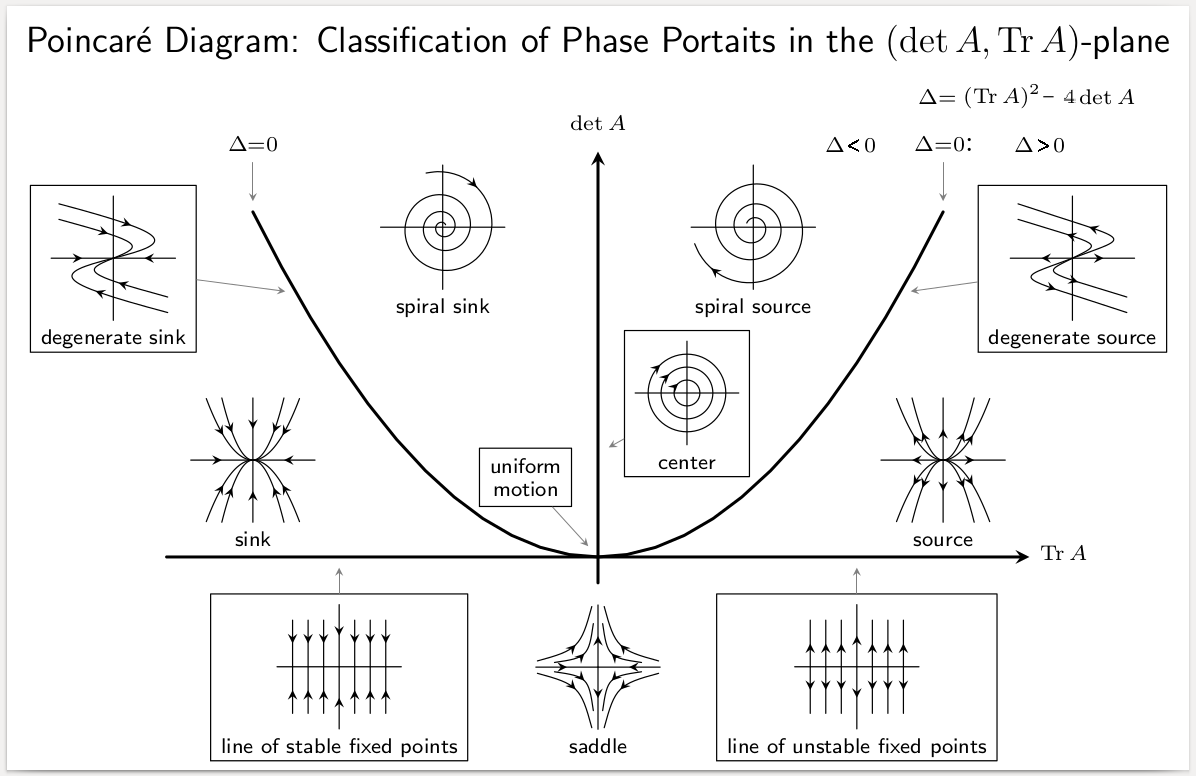
\includegraphics[width=13cm]{math_pics/Stability_Diagram.png}
\centering
\caption{Poincaré Diagram}
\end{figure}

\newpage
Taking the same concept and applying it to non-linear systems we would have:

For a non-linear autonomous system we can look at a zoomed-in portion of whichever equilibrium points we have and we may be able to locally approximate their stabilty by means of the Taylor series at that particular point, which would infer the stabilty of that point in the greater context of the non-linear system.

So for a system \ref{auton_sys_compact}
\[
\dot{y}(t) = \underline{f}(y(t)).
\] that has a fixed point $y_f \implies \underline{f}(y_f) = 0$:

If $f \in C^\infty(\mathbb{R}^n) $, the Taylor about $y_f$:
\begin{equation}\label{eq:t_taylor_expansion}
\underline{f}(y) = \underline{f}(y_f) + \left. \frac{d \underline{f}}{dy} \right|_{y_f}(y - y_f) + \mathfrak{H}(y - y_f) = J_{\underline{f}}(y_f)(y - y_f) + \mathfrak{H}(y - y_f) \tag{Taylor}
\end{equation}

$\mathfrak{H}$ is the rest of Taylor's terms which, for values near the one we're analysing can be neglected since everything looks like a line when you're that zoomed-in eitherway.

$J_{\underline{f}}(y_f)$ is the Jacobian matrix of $\underline{f}$ evaluated at point $y_f$.

\textbf{Reminder:}
\begin{definition}
The Jacobian matrix of a vector-valued vector function $f : D \subseteq \mathbb{R}^n \rightarrow S \subseteq \mathbb{R}^m$, $f(x_1, \dots, x_n) = (y_1, \dots , y_m) \quad [f(x) = (y_1, \dots , y_m)], f \in \mathcal{D}(\mathbb{R}^n)$ is $J_f \in \mathcal{M}_{m \bigtimes n}(\mathbb{R})$ an analogue for its first-order derivative, defined as:
\begin{align*}
	J_f = \left[ \frac{\partial f}{\partial x_1}, \dots , \frac{\partial f}{\partial x_n}  \right] =
	\begin{bmatrix*}
		\frac{\partial y_1}{\partial x_1} & \dots & \frac{\partial y_1}{\partial x_n} \\
		\vdots & \ddots & \vdots \\
		\frac{\partial y_m}{\partial x_1} & \dots &  \frac{\partial y_m}{\partial x_n}
	\end{bmatrix*} =
	\frac{df}{dx} =
	\left(   \frac{\partial y_i}{\partial x_j} \right)_{ij | 1 \leqslant i \leqslant n, 1 \leqslant j \leqslant m}
\end{align*}
\end{definition}

\newcommand\eqCuzOfSys{\stackrel{\mathclap{\normalfont\mbox{\ref{auton_sys_compact}}}}{=\joinrel=\joinrel=}}

Using the change of variables $\zeta = y - y_f$ and (\ref{eq:t_taylor_expansion}):
\begin{gather*}
\dot{\zeta} = \dot{y} \eqCuzOfSys \underline{f}(y) \approx J_{\underline{f}}(y_f)(\zeta) \\
\Updownarrow
\end{gather*}
\vspace*{-16mm}
\begin{gather}\label{eq:lin_approx}
\dot{\zeta} \approx J_{\underline{f}}(y_f)(\zeta). \tag{Lin. Approx.}
\end{gather}

To obtain the system's linear estimate at the fixed point $y_f$, which approximates $\underline{f}(y)$ better as $y \rightarrow y_f$.

\begin{theorem}
If $\exists J_{\underline{f}}^{-1}(y_f) \implies y_f$ is an \textbf{isolated eq. point}.
\end{theorem}

\newpage

\textbf{Proof:}
Let's try proving the flip-side of this;

Assume  $\exists J_{\underline{f}}^{-1}(y_f)$ and $y_f$ is not isolated $\implies$

$ \implies \exists y'_f \neq y_f : \underline{f}(y'_f) = 0, \norm{y_f - y'_f} < \epsilon , \forall \epsilon > 0$.

Then, taking (\ref{eq:t_taylor_expansion}) about $y'_f$ and the var. change $\zeta = y - y'_f \implies \dot{\zeta} \approx J_{\underline{f}}(y'_f)(\zeta). $

But because $f(y'_f) =0 \implies J_{\underline{f}}(y'_f)(\zeta) = 0$ and since the substitution has to hold $\forall y : \norm{y - y'_f} < \epsilon$, including $\norm{y - y'_f}|_{y \equiv y_f} > 0 \implies J_{\underline{f}(y'_f)} = 0
\quad \lightning \quad \exists J_{\underline{f}}^{-1}(y'_f)$" \qed

\vspace{20pt}
However, $\exists J_{\underline{f}}^{-1}(y_f) \nLeftarrow y_f$, in general.

Unfortunately, though, using this method we can only find the stabilty of a subclass of equilibrium points and non-linear systems.

So for a nonlinear system $\dot{y} = \underline{f}(y)$ and its (\ref{eq:lin_approx}) $\dot{\zeta} = J(y_f)\zeta$ about fixed state $y_f$ we can only show if (in the context of the non-linear system) that fixed point is either:

1.\textbf{Asymptotically stable} if $Re(\lambda) < 0, \forall \lambda \in Eig(J(y_f))$ (where $Eig(A)$ is the set of all eigenvalues of the matrix A).

2.\textbf{Unstable} if $\exists \lambda \in Eig(J(y_f)) : Re(\lambda)> 0$.

i.e. One can only show Asymptotic (or in-) stabilty, although in the case:

$Re(\lambda) \leqslant  0 \forall \lambda \in Eig(J(y_f)) \text{ and,
at least } \exists \lambda : Re(\lambda) = 0$ then the results are
inconclusive and can't be implied for the non-linear system.

\hfill\break
//TODO: HAI MA CA NU ESTI PROST invata si despre lyapuov mai bine sa

poti sa vorbesti despre dansul dupa ce zici din astea mai de
specifice de chimie ca sigur o sa ajute cu ceva na pana mea

5. arata poza de clasificarea sistemelor, dat

\hfill\break
But another way of analysing the stabilty would be by using one of
the most fundamental tools during our study, so we'll define and show
how to obtain:

\textbf{The Routh-Hurwitz matrix and its determinants.}

English mathematician Edward John Routh was looking at the
(\ref{eq:lin_approx}) of
\[
x_i' = f_i(x_1,\dots , x_n), \quad i = \overline{1,n}
\]
Namely:
\[
x_i' =\sum_{j=1}^{n}a_{ij} x_j, \quad a_{ij} = \frac{\partial
f_i}{\partial x_j}(0)
\]
He figured out he doesn't have to find the roots of
\begin{equation}\label{lin_apporx_char_equation}
det(J - \lambda I_n) =
a_0 \lambda^n + a_1 \lambda^{n-1} + \dots + a_{n-1}\lambda + a_n = 0
\end{equation}
To infer the system's stability, as in check
$ Re(\lambda_0) < 0$,

but can instead instead just simply look at the coefficients of
\ref{lin_apporx_char_equation}: $a_{i}$ to verify it.

To do this he used:

\rom{1}: Cauchy's argument principle

and

\rom{2}: Sturm's theorem

\rom{1}

Cauchy's argument principle states that for the poly. $p \in \mathbb{C}[Z]$:
\[
p(z) = u(z) + i v(z), \quad u, v \in \mathbb{R}[Z]; u,v : \mathbb{C}
\rightarrow \mathbb{R}
\]
Its number of roots inside a closed contour $\gamma$  is $=$ to the
number of positive rotations (counter-clockwise)[c.c.] that $(u(z),
v(z))$ (or $arg(p(z))$) makes as $z$ moves across $\partial \gamma$
in a positive sense [c.c.].

\hfill\break
//TODO: ai putea sa pui si tu o poza cu un vector space format de un
\hfill\break

anumit polinom complex cu valori complexe

Now all we need to do is make this "closed contour" the entire
left-half of the complex axis!

We could write it as a {\large HUGE} half-circle
\[
z = Re^{i \theta}, \quad \frac{\pi}{2} \leq \theta \leq \frac{3
\pi}{2}, R \text{ sufficiently large }
\]

The thing is even if it's the case that all $n$ roots lie inside it,
$arg(p(z))$ will only make $\frac{n}{2}$ rotations since this is a
half circle, so we could combine this fact with a more elegant way of
writing "the half-plane, left of the imaginary axis" into:

\begin{lemma}\label{cauchy_arg_lemma}
For $p(z) \in \mathbb{C}_n[Z]$ and $p(ix) \neq 0. \forall x \in
\mathbb{R}$. Then $\forall z_0 : p(z_0) = 0, Re(z_0) < 0 \iff$
$arg(p(ix))$ makes $\frac{n}{2}$ positive rotations for $x \in
[-\infty , \infty]$.
\end{lemma}

\rom{2}.

The second tool he's used was Sturm's theorem, which was the result
of his discovery that for the division $\frac{p_{i-1}(x)}{p_i(x)}$,
for $p_k \in \mathbb{R}[X]$ it's better to take the remainder
$p_{i+1}(x)$ with a negative sign:
\begin{equation}\label{euclid_algorithm}
p_{i-1}(x) = p_i(x) q_i(x) - p_{i+1}(x) \tag{Euclid's Algorithm}
\end{equation}
Because, if we do that, then:
\begin{equation}\label{sturm_seq_property}
\text{sign} ( p_{i+1}(x) )  \neq \text{sign} ( p_{i-1}(x) ), \quad
\text{for} \quad p_i(x)=0 \tag{Sturm. Seq. Property}
\end{equation}
This is called the "Sturm sequence property"

And if we construct a sequence
\[
(p_k)_{k = \overline{0,m}} \subset \mathbb{R}[X]
\]
and the function
\begin{gather}\label{no_sign_changes_func}
w : \mathbb{R} \rightarrow \mathbb{R} \notag  \\
w(x) = \text{No. of sign changes of  } (p_k)(x) \notag
\end{gather}
Then we find that for:
\begin{gather*}
p_i^{-1}(0) \text{ ( set of roots for $p_i$) } \\
R := \bigcup_{i \in \left\{ 1, \dots, m-1 \right\} } p_i^{-1}(0) \\
\forall x_1, x_2 \in R, w(x_1) = w(x_2)
\end{gather*}
Hence we have:
\begin{lemma}\label{sturm_lemma}
For a seq. of $  (p_k)_{k = \overline{0,m}} \subset \mathbb{R}[X]$
that satifies:

\rom{1}
$ deg(p_0) > deg(p_1), $

\rom{2}
$\nexists x \in \mathbb{R} : p_0(x) = p_1(x) = 0, $

\rom{3}
$p_m(x) \neq 0, \forall x \in \mathbb{R}$

\rom{4}
And (\ref{sturm_seq_property})
\par
We have (for the above defined $w$ \ref{no_sign_changes_func}) :
\begin{gather}
	\frac{w(\infty) - w(-\infty)}{2} =  \notag \\
	\text{No. of positive rotations of the vector } \notag \\
	(p_0(x), p_1(x)), \text{as $x$ tends from  } x \in [-\infty, +\infty] \notag
\end{gather}
\end{lemma}

Proof: As stated in \ref{sturm_seq_property}: $w(x)$ doesn't change at roots of

$p_k(x), k = \overline{1,m-1}$. Asumption \rom{3} shows $p_m(x)$
doesn't influence it either. So there can only be one suspect:
$p_0(x)$. If there's a spike by $1$ at $\overline{x}$ in $w(\overline{x})$,

zero of $p_0$
(   $p_0(\overline{x}) =0 $) either:
\[
p_0(x) \text{ changes from + to - and   } p_1(\overline{x}) > 0
\]
or:
\[
p_0(x) \text{ changes from - to + and  } p_1(\overline{x}) < 0
\]
[   $\nexists \overline{x}: p_1(\overline{x}) = 0$ by assumption \rom{2}  ]

Both of which cause the vector $(p_0(x), p_1(x))$ to cross the
imaginary axis in a positive sense.

If there's a dip in $w$ at $\overline{x}$, however, the crossing is
done clock-wise, this time.

Now taking \rom{1} into account and the fact that $(p_0(y), p_1(y))$
is horizontal for $y \rightarrow  - \infty$ and $y \rightarrow +
\infty  $ outcomes the result of our lemma
\qed

\hfill\break
//TODO Maybe try to draw this yourself cu arrows nstuff
\hfill\break

\begin{figure}
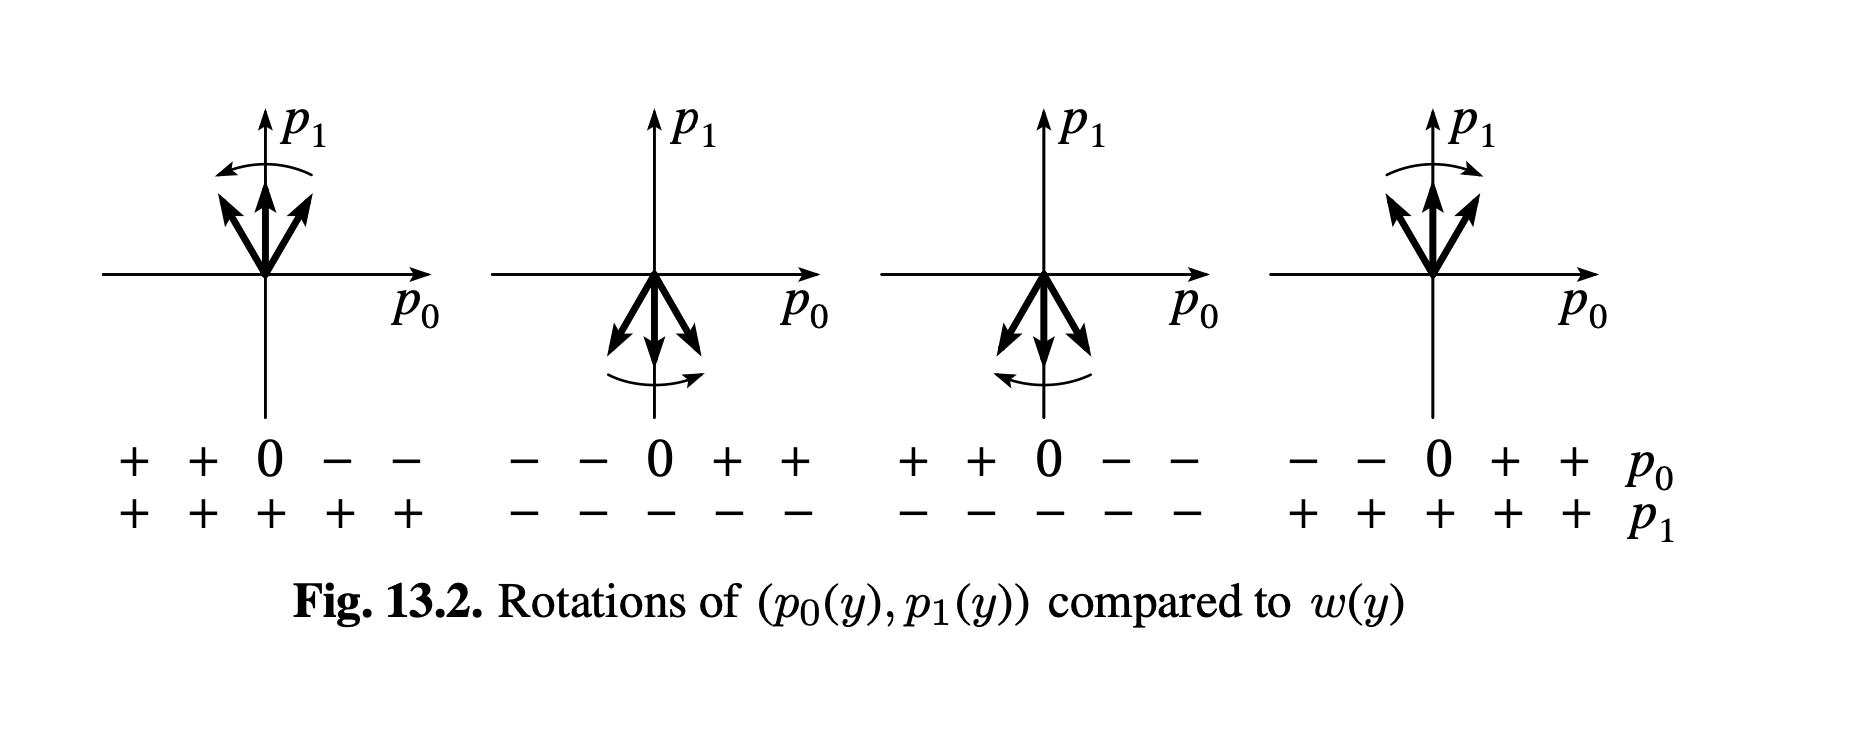
\includegraphics[width=13cm]{math_pics/sageti-cumse-invart.png}
\centering
\end{figure}

So using these 2 Lemmas we have the criteria for stabilty:
For the characteristic polynomial \ref{lin_apporx_char_equation},
written instead like this:
\[
p(z)=a_0 z^n + a_1z^{n-1} + \dots + a_n = 0, \quad a_0 > 0
\]

Dividing $\frac{p(i x)}{i^n}$ and using \ref{real_imag_another_way_to_write}
\begin{gather}
p_0(x)= \text{Re}(\frac{p(i x)}{i^n}) = a_0 x^{n} -a_2 x^{n-2} + a_4
x^{n-4} \pm \dots \\
p_1(x)= -\text{Im} (\frac{p(i x)}{i^n}) = a_1 x^{n-1} -a_3 x^{n-3} +
a_5 x^{n-5} \pm \dots
\end{gather}

More generally:
\begin{equation}\label{polys_general_form}
p_i(x) = c_{i0} x^{n-i} + c_{i1} x^{n-i-2} + c_{ i2 } x^{ n-i-4  } +
\dots, \tag{Gen. Form}
\end{equation}

And $q_i(x) = (  \frac{c_{ i-1 ,0}}{c_{ i0 }} )x$ from
\ref{euclid_algorithm} given that $c_{i0} \neq 0$.
Putting \ref{polys_general_form} into \ref{euclid_algorithm} to get
the general form of all the coefficients as well we get:
\begin{align}\label{coeff_gen_form}
c_{i+1,j} = c_{i,j+1} \cdot \frac{c_{i-1,0}}{c_{i,0}} - c_{i-1,j+1 }
= \frac{1}{c_{i,0}} \text{det}
\begin{pmatrix}
	c_{i-1,0} & c_{i-1, j+1}            \\
	c_{i,0}   & c_{i, j+1} \tag{Coeff.}
\end{pmatrix}
\end{align}

The algo. stops for $ p_m(x) $ with $ m < n$ if $c_{i,0} = 0$ at a
particular $i \implies q_i(x)$ is of higher degree.

And so: $(p_i(x))_{i = \overline{1,m \text{ or } n}}$ verifies
\rom{1}, \rom{4} from \ref{sturm_lemma}

\rom{2} $\iff p(ix) \neq 0, \forall x \in \mathbb{R}$

$p_m(x) = \text{gcd}(p_0(x), p_1(x)) \iff \text{ \rom{2} } \implies
\text{ \rom{3} }$

\par

So here's the big guy:

\begin{theorem}\label{routh_theorem}
Routh:
\begin{gather*}
	Re(\lambda) < 0, \quad \forall \lambda \in \text{det}(J - \lambda
	I_n)^{-1}(0) \text{ from \ref{lin_apporx_char_equation} with } a_0 > 0 \\
	\Updownarrow  \\
	c_{i,0} > 0, \forall  i = \overline{1,n} \text{ from \ref{coeff_gen_form} }
\end{gather*}
\end{theorem}
Meaning the system is stable.

\textbf{Proof: } $arg(p_0,p_1) = 360^\degree - arg(\text{Re}(p),
\text{Im}(p)) \implies \frac{n}{2}$ positive rotations of $p(ix)$ are
bascially $\frac{n}{2}$ neg. rot. of $(p_0(x), p_1(x))$. If
$Re(\lambda) < 0, \forall \lambda \in p(\lambda)^{-1}(0) \implies$ (
from  \ref{cauchy_arg_lemma}, \ref{sturm_lemma} ) $w(\infty) - w( -
\infty) = -n$. Could only be for $w(\infty) = 0, w(- \infty) = n$,
though. $ \implies p_i(x) \geq 0$ for all leading $i$. Having
\ref{routh_theorem} $\implies p_n(x) \equiv c_{n0}$. Because
$\nexists \text{gcd}(p_0(x),p_1(x)), p(\lambda) \neq 0$ for
Re$(\lambda) = 0$. Now we just do \ref{cauchy_arg_lemma} +
\ref{sturm_lemma} once more. \qed

\hfill\break
//TODO vezi ba sa rezolbi asta cumva ca nu esti chiar asa prost te pui cu pixu cu astea sa vezi de unde vine si faci pasii de rezolvare de le-a facut hurwitz intr-un fel
\hfill\break

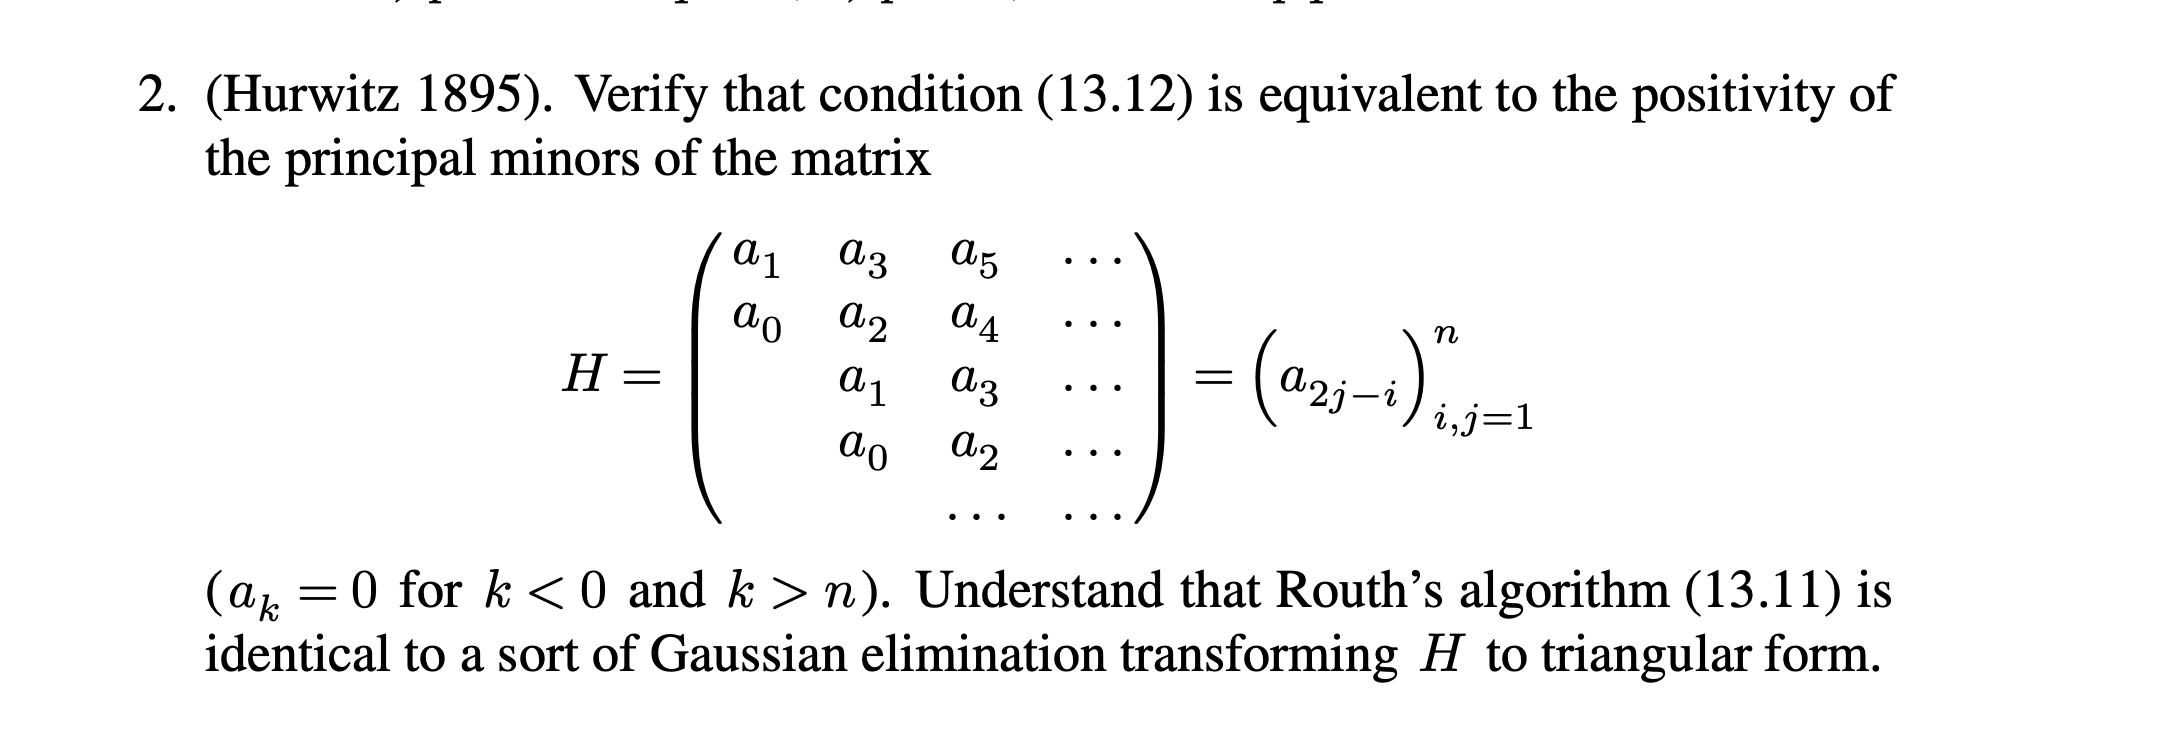
\includegraphics[width=13cm]{math_pics/TODO SA FACI KKTU ASTA BA.png}

Adolf Hurwitz later wrote the positivity criterion ($2^{nd}$ condition in \ref{routh_theorem}) making use of this matrix we now basically call "his".
\newpage
\begin{theorem}\label{hurwitz_theorem}
Hurwitz:

We have \ref{lin_apporx_char_equation}
\[
	p(\lambda) = a_0 \lambda^n + a_1 \lambda^{n-1} + \dots + a_{n-1}\lambda + a_n = 0
\]

and constructing its \textbf{Hurwitz matrix}:
\begin{align*}
	H_n =
	\begin{pmatrix*}
		a_{2i-j}
	\end{pmatrix*}^n_{i,j=1} =
	\begin{pmatrix*}
		a_1 & a_0 & 0 & 0 & 0 & \dots & 0 \\
		a_3 & a_2 &  a_1 & a_0 & 0 & \dots &  0 \\
		\vdots & \vdots & \vdots & \vdots & \vdots & \ddots & \vdots \\
		a_{ 2n-1 } &  a_{ 2n-2 } & a_{ 2n-3 }  & a_{ 2n-4 }  & a_{ 2n-5 }  & \dots & a_n
	\end{pmatrix*}
\end{align*}

with the exception that $a_k = 0$ if $k \notin \left\{0, \dots , n\right\}$

He's shown that condition \rom{2} of \ref{routh_theorem} (hence $\text{ Re }(\lambda)< 0, \forall \lambda \in p^{-1}(0)$ with $a_0 > 0$ as well) $\iff \text{det}(H_i) \forall i = \overline{1,n}$

So this is what's used to show the stabilty of the linear system (or linearization of a non-linear one), computing matrices of coefficients of the charracteristic polynomial, instead of having to compute Eig($J$) directly.
\end{theorem}

We'll use this later during the section about \text{bifurcations} as well.

\vskip\bigskipamount
